\documentclass{article}

\usepackage{graphicx}
\usepackage{pythontex}
\setpythontexworkingdir{.}
\usepackage{tikz} % for drawing
\usepackage{pgfplotstable}
\usetikzlibrary{pgfplots.groupplots}

\title{test}
\begin{document}
\maketitle

Here is text. Below are some plots.
Why does it auto not recompile?
More text, and more, why is it not compiling
vel vel

\begin{figure}[h]
\centering
\begin{pycode}
import matplotlib.pyplot as plt
import tikzplotlib
plt.plot([1, 2, 3, 4, 5], [4, 5, 2, 4, 1], label="x")
plt.legend()
print(tikzplotlib.get_tikz_code(axis_height="5cm", axis_width="6cm"))
plt.clf()
\end{pycode}
\caption{It works very well.}
\end{figure}

\begin{figure}[h]
\centering
\begin{pycode}
import matplotlib.pyplot as plt
import tikzplotlib
plt.figure()
plt.subplot(121)
plt.plot([1, 2, 3, 4, 5], [4, 5, 2, 4, 1], label="x")
plt.legend()
plt.subplot(122)
plt.plot([1, 2, 3, 4, 5], [8, 7, 6, 5, 4], label="y")
plt.legend()
print(tikzplotlib.get_tikz_code(axis_height="6cm"))#%axis_height="5cm", axis_width="7cm"))
plt.clf()
\end{pycode}
\caption{Subplots in action.}
\end{figure}

\begin{figure}
\centering
\begin{pycode}
import plot
plot.plot1()
print(tikzplotlib.get_tikz_code(axis_height="5cm", axis_width="6cm"))
plt.clf()
\end{pycode}
\caption{Second fig}
\end{figure}

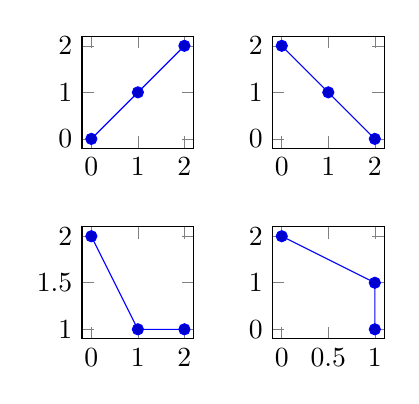
\begin{tikzpicture}
  \begin{groupplot}[group style={group size=2 by 2},height=3cm,width=3cm]
    \nextgroupplot
    \addplot coordinates {(0,0) (1,1) (2,2)};
    \nextgroupplot
    \addplot coordinates {(0,2) (1,1) (2,0)};
    \nextgroupplot
    \addplot coordinates {(0,2) (1,1) (2,1)};
    \nextgroupplot
    \addplot coordinates {(0,2) (1,1) (1,0)};      
  \end{groupplot}
\end{tikzpicture}
% Same example created as done without the library
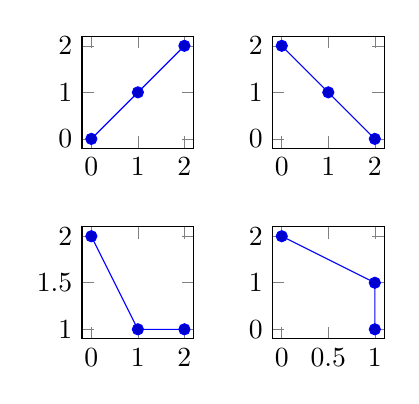
\begin{tikzpicture}
  \begin{axis}[name=plot1,height=3cm,width=3cm]
    \addplot coordinates {(0,0) (1,1) (2,2)};
  \end{axis}
  \begin{axis}[name=plot2,at={($(plot1.east)+(1cm,0)$)},anchor=west,height=3cm,width=3cm]
    \addplot coordinates {(0,2) (1,1) (2,0)};
  \end{axis}
  \begin{axis}[name=plot3,at={($(plot1.south)-(0,1cm)$)},anchor=north,height=3cm,width=3cm]
    \addplot coordinates {(0,2) (1,1) (2,1)};
  \end{axis}
  \begin{axis}[name=plot4,at={($(plot2.south)-(0,1cm)$)},anchor=north,height=3cm,width=3cm]
    \addplot coordinates {(0,2) (1,1) (1,0)};
  \end{axis}
\end{tikzpicture}

\end{document}
